\documentclass[tikz=true]{standalone}
\usepackage{graphicx, standalone}
\usepackage[compat=1.1.0]{tikz-feynman}
\usepackage{tikz}
\usepackage{amsmath, amssymb}
\usepackage{euler}
\usepackage{fontspec}
\setmainfont{MinionPro}
\usepackage{comment}

\renewcommand{\k}{\ensuremath\text{k}}
\newcommand{\kp}{\ensuremath\text{k}'}
\newcommand{\q}{\ensuremath\text{q}}

\begin{document}

% LEFT HAND SIDE
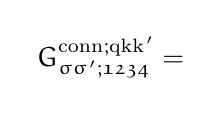
\begin{tikzpicture}[baseline=(current bounding box.center)]
	\node {$G_{\sigma\sigma';\mathfrak{1234}}^{\text{conn};\q\k\kp}=$};
\end{tikzpicture}

% DIAGRAM 1
\begin{tikzpicture}[baseline=(current bounding box.center)]
    \node {$-$};
\end{tikzpicture}
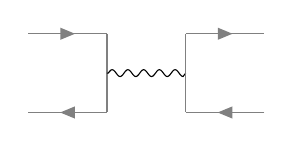
\begin{tikzpicture}[baseline=(current bounding box.center)]
	\begin{feynman}[small]
		\vertex (a1);
		\vertex[right=of a1] (b1);
		\vertex[below=of b1] (b3);
		\vertex[left=of b3] (a2);
		
		\path (b1) -- (b3) coordinate[midway] (b2);	
						
		\vertex[right=of b1] (c1);
		\vertex[below=of c1] (c3);
		\vertex[right=of c1] (d1);
		\vertex[right=of c3] (d2);
		
		\path (c1) -- (c3) coordinate[midway] (c2);	
		
		\diagram* {
			(a1) -- [fermion, gray] (b1) -- [gray] (b3) -- [fermion, gray] (a2),
			(b2) -- [photon] (c2),
			(d2) -- [fermion, gray] (c3) -- [gray] (c1) -- [fermion, gray] (d1)
		};	
	\end{feynman}
\end{tikzpicture}

% DIAGRAM 2
\begin{tikzpicture}[baseline=(current bounding box.center)]
    \node {$+$};
\end{tikzpicture}
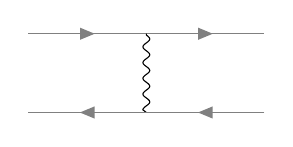
\begin{tikzpicture}[baseline=(current bounding box.center)]
	\begin{feynman}[small]
		\vertex (a1);
		\vertex[below=of a1] (a2);
		\vertex[right=1.5cm of a1] (b1);
		\vertex[below=of b1] (b2);
		\vertex[right=1.5cm of b1] (c1);
		\vertex[below=of c1] (c2);
		
		\diagram* {
			(a1) -- [fermion, gray] (b1) -- [fermion, gray] (c1),
			(b1) -- [photon] (b2),
			(c2) -- [fermion, gray] (b2) -- [fermion, gray] (a2)
		};	
	\end{feynman}
\end{tikzpicture}

% DIAGRAM 3
\begin{tikzpicture}[baseline=(current bounding box.center)]
    \node {$-$};
\end{tikzpicture}
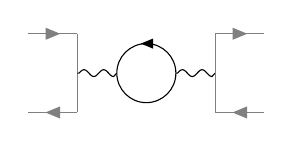
\begin{tikzpicture}[baseline=(current bounding box.center)]
	\begin{feynman}[small]
		\vertex (a1);
		\vertex[right=0.625cm of a1] (b1);
		\vertex[below=of b1] (b3);
		\vertex[below=of a1] (a3);		
		\path (b1) -- (b3) coordinate[midway] (b2);	
		
		
		\vertex[right=0.5cm of b2] (c2);
		\vertex[right=0.75cm of c2] (d2);
		\vertex[right=0.5cm of d2] (e2);
		\vertex[right=1.75cm of b1] (e1);
		\vertex[below=of e1] (e3);
		\vertex[right=0.625cm of e1] (f1);
		\vertex[below=of f1] (f3);
		
		\path (e1) -- (e3) coordinate[midway] (e2);	
		
		\def\r{0.375}
		
		\path (c2) -- (d2) coordinate[midway] (A);
		\draw[fermion, arrow size=1pt, transform canvas={rotate around={-90:(A)}}] 
        (A) circle (\r);
		
		\diagram* {
			(a1) -- [fermion, gray] (b1) -- [gray] (b3) -- [fermion, gray] (a3),
			(b2) -- [photon] (c2),
			(d2) -- [photon] (e2),
			(f3) -- [fermion, gray] (e3) -- [gray] (e1) -- [fermion, gray] (f1)
		};	
	\end{feynman}
\end{tikzpicture}

% DIAGRAM 4
\begin{tikzpicture}[baseline=(current bounding box.center)]
    \node {$-$};
\end{tikzpicture}
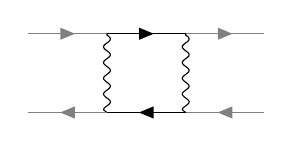
\begin{tikzpicture}[baseline=(current bounding box.center)]
	\begin{feynman}[small]
		\vertex (a1);
		\vertex[below=of a1] (a2);
		\vertex[right=of a1] (b1);
		\vertex[below=of b1] (b2);
		\vertex[right=of b1] (c1);
		\vertex[right=of b2] (c2);
		\vertex[right=of c1] (d1);
		\vertex[right=of c2] (d2);
		
		\diagram* {
			(a1) -- [fermion, gray] (b1) -- [fermion] (c1) -- [fermion, gray] (d1),
			(b1) -- [photon] (b2),
			(d2) -- [fermion, gray] (c2) -- [fermion] (b2) -- [fermion, gray] (a2),
			(c1) -- [photon] (c2),
		};	
	\end{feynman}
\end{tikzpicture}

% DIAGRAM 5
\begin{tikzpicture}[baseline=(current bounding box.center)]
    \node {$+$};
\end{tikzpicture}
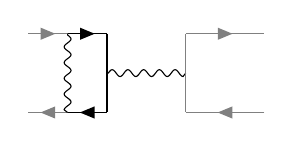
\begin{tikzpicture}[baseline=(current bounding box.center)]
	\begin{feynman}[small]
		\vertex (a1);
		\vertex[right=of a1] (b1);
		\vertex[below=of b1] (b3);
		\vertex[left=of b3] (a3);
		
		\path (b1) -- (b3) coordinate[midway] (b2);
		\path (a1) -- (b1) coordinate[midway] (i1);	
		\path (a3) -- (b3) coordinate[midway] (i3);	
						
		\vertex[right=of b1] (c1);
		\vertex[below=of c1] (c3);
		\vertex[right=of c1] (d1);
		\vertex[right=of c3] (d3);
		
		\path (c1) -- (c3) coordinate[midway] (c2);	
		\path (c1) -- (d1) coordinate[midway] (j1);	
		\path (c3) -- (d3) coordinate[midway] (j3);
		
		\diagram* {
			(a1) -- [fermion, gray] (i1) -- [fermion] (b1) -- (b3) -- [fermion] (i3) -- [fermion, gray] (a3),
			(b2) -- [photon] (c2),
			(i1) -- [photon] (i3),
			(d3) -- [fermion, gray] (c3) -- [gray] (c1) -- [fermion, gray] (d1)
		};	
	\end{feynman}
\end{tikzpicture}

% DIAGRAM 6
\begin{tikzpicture}[baseline=(current bounding box.center)]
    \node {$+$};
\end{tikzpicture}
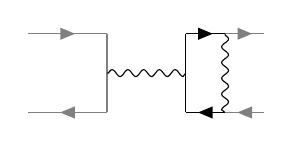
\begin{tikzpicture}[baseline=(current bounding box.center)]
	\begin{feynman}[small]
		\vertex (a1);
		\vertex[right=of a1] (b1);
		\vertex[below=of b1] (b3);
		\vertex[left=of b3] (a3);
		
		\path (b1) -- (b3) coordinate[midway] (b2);
		\path (a1) -- (b1) coordinate[midway] (i1);	
		\path (a3) -- (b3) coordinate[midway] (i3);	
						
		\vertex[right=of b1] (c1);
		\vertex[below=of c1] (c3);
		\vertex[right=of c1] (d1);
		\vertex[right=of c3] (d3);
		
		\path (c1) -- (c3) coordinate[midway] (c2);	
		\path (c1) -- (d1) coordinate[midway] (j1);	
		\path (c3) -- (d3) coordinate[midway] (j3);
		
		\diagram* {
			(a1) -- [fermion, gray] (b1) -- [gray] (b3) -- [fermion, gray] (a3),
			(b2) -- [photon] (c2),
			(j1) -- [photon] (j3),
			(d3) -- [fermion, gray] (j3) -- [fermion] (c3) -- (c1) -- [fermion] (j1) -- [fermion, gray] (d1)
		};	
	\end{feynman}
\end{tikzpicture}

% DIAGRAM 7
\begin{tikzpicture}[baseline=(current bounding box.center)]
    \node {$+$};
\end{tikzpicture}
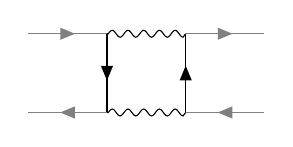
\begin{tikzpicture}[baseline=(current bounding box.center)]
	\begin{feynman}[small]
		\vertex (a1);
		\vertex[below=of a1] (a2);
		\vertex[right=of a1] (b1);
		\vertex[below=of b1] (b2);
		\vertex[right=of b1] (c1);
		\vertex[right=of b2] (c2);
		\vertex[right=of c1] (d1);
		\vertex[right=of c2] (d2);
		
		\diagram* {
			(a1) -- [fermion, gray] (b1) -- [fermion] (b2) -- [fermion, gray] (a2),
			(b1) -- [photon] (c1),
			(d2) -- [fermion, gray] (c2) -- [fermion] (c1) -- [fermion, gray] (d1),
			(b2) -- [photon] (c2),
		};	
	\end{feynman}
\end{tikzpicture}

% DIAGRAM 8
\begin{tikzpicture}[baseline=(current bounding box.center)]
    \node {$+$};
\end{tikzpicture}
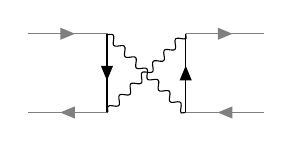
\begin{tikzpicture}[baseline=(current bounding box.center)]
	\begin{feynman}[small]
		\vertex (a1);
		\vertex[below=of a1] (a2);
		\vertex[right=of a1] (b1);
		\vertex[below=of b1] (b2);
		\vertex[right=of b1] (c1);
		\vertex[right=of b2] (c2);
		\vertex[right=of c1] (d1);
		\vertex[right=of c2] (d2);
		
		\diagram* {
			(a1) -- [fermion, gray] (b1) -- [fermion] (b2) -- [fermion, gray] (a2),
			(b1) -- [photon] (c2),
			(d2) -- [fermion, gray] (c2) -- [fermion] (c1) -- [fermion, gray] (d1),
			(b2) -- [photon] (c1),
		};	
	\end{feynman}
\end{tikzpicture}

% DIAGRAM 9
\begin{tikzpicture}[baseline=(current bounding box.center)]
    \node {$-$};
\end{tikzpicture}
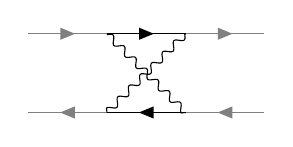
\begin{tikzpicture}[baseline=(current bounding box.center)]
	\begin{feynman}[small]
		\vertex (a1);
		\vertex[below=of a1] (a2);
		\vertex[right=of a1] (b1);
		\vertex[below=of b1] (b2);
		\vertex[right=of b1] (c1);
		\vertex[right=of b2] (c2);
		\vertex[right=of c1] (d1);
		\vertex[right=of c2] (d2);
		
		\diagram* {
			(a1) -- [fermion, gray] (b1) -- [fermion] (c1) -- [fermion, gray] (d1),
			(b1) -- [photon] (c2),
			(d2) -- [fermion, gray] (c2) -- [fermion] (b2) -- [fermion, gray] (a2),
			(c1) -- [photon] (b2),
		};	
	\end{feynman}
\end{tikzpicture}

% DIAGRAM 10
\begin{tikzpicture}[baseline=(current bounding box.center)]
    \node {$-$};
\end{tikzpicture}
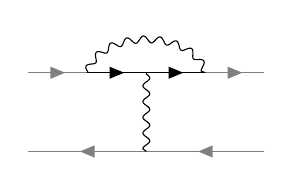
\begin{tikzpicture}[baseline=(int.center)]
	\begin{feynman}[small]
		\vertex (a1);
		\vertex[right=1.5cm of a1] (b1);
		\vertex[right=1.5cm of b1] (c1);
		
		\vertex[below=of a1] (a2);
		\vertex[below=of b1] (b2);
		\vertex[below=of c1] (c2);
		
		\path (a1) -- (b1) coordinate[midway] (i1);
		\path (b1) -- (c1) coordinate[midway] (i2);
		
		\path (b1) -- (b2) coordinate[midway] (int);
		
		\diagram* {
			(a1) -- [fermion, gray] (i1) -- [fermion] (b1) -- [fermion] (i2) -- [fermion, gray] (c1),
			(i1) -- [photon, bend left=75] (i2),
			(c2) -- [fermion, gray] (b2) -- [fermion, gray] (a2),
			(b1) -- [photon] (b2)
		};	
	\end{feynman}
\end{tikzpicture}

% DIAGRAM 11
\begin{tikzpicture}[baseline=(current bounding box.center)]
    \node {$-$};
\end{tikzpicture}
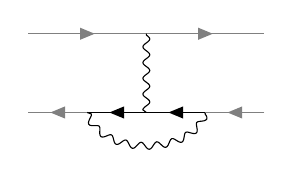
\begin{tikzpicture}[baseline=(int.center)]
	\begin{feynman}[small]
		\vertex (a1);
		\vertex[right=1.5cm of a1] (b1);
		\vertex[right=1.5cm of b1] (c1);
		
		\vertex[below=of a1] (a2);
		\vertex[below=of b1] (b2);
		\vertex[below=of c1] (c2);
		
		\path (a2) -- (b2) coordinate[midway] (i1);
		\path (b2) -- (c2) coordinate[midway] (i2);
		
		\path (b1) -- (b2) coordinate[midway] (int);
		
		\diagram* {
			(a1) -- [fermion, gray] (b1) -- [fermion, gray] (c1),
			(i2) -- [photon, bend left=75] (i1),
			(c2) -- [fermion, gray] (i2) -- [fermion] (b2) -- [fermion] (i1) -- [fermion, gray] (a2),
			(b1) -- [photon] (b2)
		};	
	\end{feynman}
\end{tikzpicture}

% DIAGRAM 12
\begin{tikzpicture}[baseline=(current bounding box.center)]
    \node {$+$};
\end{tikzpicture}
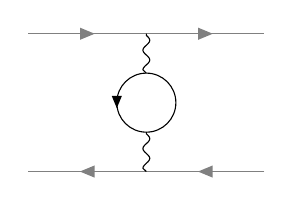
\begin{tikzpicture}[baseline=(int.center)]
	\begin{feynman}[small]
		\vertex (a1);
		\vertex[right=1.5cm of a1] (b1);
		\vertex[right=1.5cm of b1] (c1);
		
		\vertex[below=0.5cm of b1] (i1);
		\vertex[below=0.75cm of i1] (i2);
		\vertex[below=0.5cm of i2] (b2);
		
		\vertex[left=1.5cm of b2] (a2);
		\vertex[right=1.5cm of b2] (c2);
		
		\path (b1) -- (b2) coordinate[midway] (int);
		
		\def\r{0.375}
		
		\path (i1) -- (i2) coordinate[midway] (A);
		\draw[fermion, arrow size=1pt] (A) circle (\r);
		
		\diagram* {
			(a1) -- [fermion, gray] (b1) -- [fermion, gray] (c1),
			(c2) -- [fermion, gray] (b2) -- [fermion, gray] (a2),
			(b1) -- [photon] (i1),
			(i2) -- [photon] (b2)
		};	
	\end{feynman}
\end{tikzpicture}

\end{document}